\documentclass[]{article}
\usepackage[utf8]{inputenc}
\usepackage[T1]{fontenc}
\usepackage[danish]{babel}
\usepackage{amsmath}
\usepackage{graphicx,wrapfig,lipsum}

\begin{document}
\tableofcontents
Hello World!
ÆØÅ
\\
sgsdgfdfdfddddddddds \quad \qquad  aofjio aiofenoi aifojna aowndoi aofjwnoa aofno aonfaoij aofje n aoa o afsda

hhhhh

Se afsnit \ref{kk} for mere info
\raggedleft{dddddd}
gggg
\\
gedgs
\raggedright
asfasfdfs \\
ageasf
\newpage

\begin{enumerate}
\item \begin{itemize}
\item ff
\end{itemize}
\end{enumerate}
%\sfrac{55}{66}
\section{Kager} \label{kk}
\begin{align}
\end{align}
\newpage
hh
\begin{figure}
\caption{Kageplanen (uden kage)}
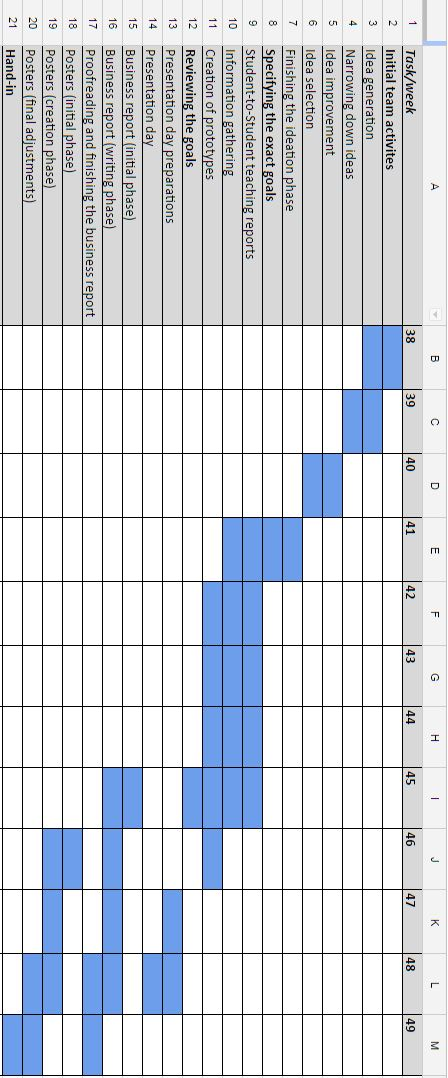
\includegraphics[scale=0.6]{Time}
\caption{Kageplanen (uden kage)}
\end{figure}


\end{document}




